\section{Galaxies}
\subsection{Questions}
galaxies suck!!!!
\begin{enumerate}
\item \textbf{Define two-body relaxation and estimate its time scale in (a) a globular cluster; (b)
      the Milky Way's disk. In which cases is two-body relaxation important?}
      
      Here's one way of calculating two-body relaxation. Assume $N$ bodies of mass $m$. Look at one mass travelling past another mass with relative velocity $v$ and impact parameter $b$. Assume that the time for the two to interact gravitationally is $2b/v$, that is, they are only interacting while the moving mass is $b$ away from its point of closest approach. The acceleration the mass feels due to the other mass is on the order of $Gm/b^2$. Therefore the change in velocity is
      \begin{equation}
      \delta v_\perp (v,b) \sim \frac{Gm2b}{b^2v} = \frac{2Gm}{bv}\,\,.
      \end{equation}
      When looking at many interactions over time, $(\delta v_\perp)^2$ grows with time.
      \begin{equation}
      \frac{d}{dt}(\delta \bar{v_\perp})^2 \sim \int^{b_{\rm max}}_{b_{\rm min}}\delta v_\perp^2(v,b) n v 2 \pi b db \sim \frac{8 \pi G^2 m^2 n}{v} \ln \biggl( \frac{b_{\rm max}}{b_{\rm min}} \biggr) \,\, .
      \end{equation}
      The factor of $n v 2 \pi b db$ comes from thinking about many masses streaming past our central mass. The flux of masses in number per second per area is $nv$. Then we can imagine a ring of radius $b$ through which the particles are streaming. It has circumference $2 \pi b$ and thickness $db$, so the area of this thin ring can be multiplied by the flux to get the number of interactions per time. Then we just multiply the rate of interactions by the squared change in velocity. We can approximate the relaxation time as
      \begin{equation}
      t_R = \frac{v^2}{\frac{d}{dt}(\delta \bar{v_\perp})^2} = \frac{v^3}{8 \pi G^2 m^2 n \ln(b_{\rm max}/b_{\rm min})} \,\,.
      \end{equation}
      Let's say $b_{\rm max} \sim R \sim (N/n)^{1/3}$, where $N$ is the total number of bodies in the system, while $b_{\rm max} \sim n^{-1/3}$. Therefore
      \begin{equation}
      \frac{b_{\rm max}}{b_{\rm min}} \sim N^{1/3}\,\,.
      \end{equation}
      
      The average density of stars in a globular cluster is $0.4~{\rm pc}^{-3}$, and we can probably assume the average mass is something like $1-2~{\rm M}_\odot$.
\item \textbf{Draw qualitatively the spectral energy distribution of the Milky Way, and describe
      how its morphology might appear to an external observer as a function of wavelength.}
      
      \begin{figure}[!h]
\begin{center}
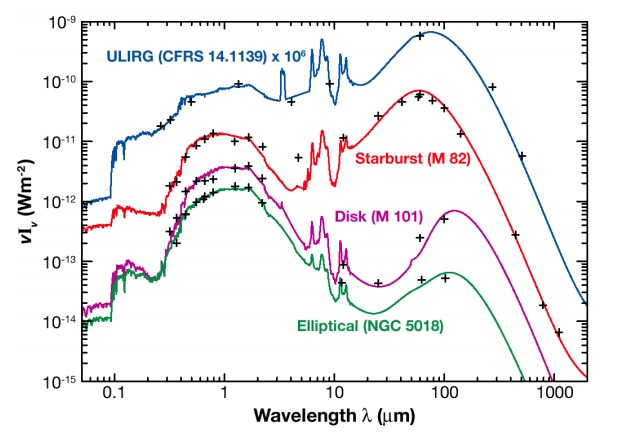
\includegraphics[width=\textwidth]{galaxy_sed.jpg}
\end{center}
\end{figure}

The spectral energy distribution of the Milky Way looks like the magenta curve on the above plot.  There are a number of important features, which will be identified by their wavelength range.  

1. $ \thicksim0.1 \mu m$:  This is the Lyman limit.  912 angstroms corresponds to the photon energy required to ionize the electron in the hydrogen ground state.  The left of the break is dominated by stars whoa re hot enough to produce many photons with 13.6 eV or more that can ionize hydrogen en masse.  This appears as a sharp break because the opacity dramatically increases when stars become hot enough to produce photons at these energies.  

2.  $\thicksim 0.1 \mu m - 0.25 \mu m$:  Here the UV continuum of the disk SED is lower than that of a star-forming galaxy since it does not have as many O and B stars that dominate this wavelength range.

3. $ 0.25 \mu m - 1 \mu m$:  Dust extinction is strong for bluer optical wavelengths (also for UV), which causes the downward slope as wavelength decreases.  The bluer the light is, the more it is extinct.

4.  $  \thicksim 1 \mu m - \thicksim 11 \mu m$:  After the peak at $1 \mu m$, which is dominated by $1 M_\odot$ and slightly lower mass stars, this wavelength range is dominated by evolved and low mass stars, which output a lower total intensity than the solar mass stars at the peak.  The longer the wavelength, the cooler the star, and the less energy is outputted.  This regime also has little to no extinction.   

5.  $\thicksim 5 \mu m - \thicksim 10 \mu m$:  These strong emission lines are due to PAHs (polycyclic aromatic hydrocarbons).  These are complex organic planar molecules with multiple benzene ring-like structures that are probably responsible for a series of molecular bonds that have been observed in emission in the light from diffuse dust clouds.  The emission lines appear to be due to vibrations in the C-C and C-H bonds common in PAHs.  

6.  $\thicksim 100 \mu m$:  Dust in the galaxy preferentially absorbs shorter wavelengths, i.e. UV and blue optical.  This peak is due to this high energy radiation being absorbed and re-emitted (i.e. reprocessed), as thermal emission by dust.


The following figure is the one to have in mind when thinking about the morphology of the Milky Way as a function of wavelength.

\begin{figure}[!h]
\begin{center}
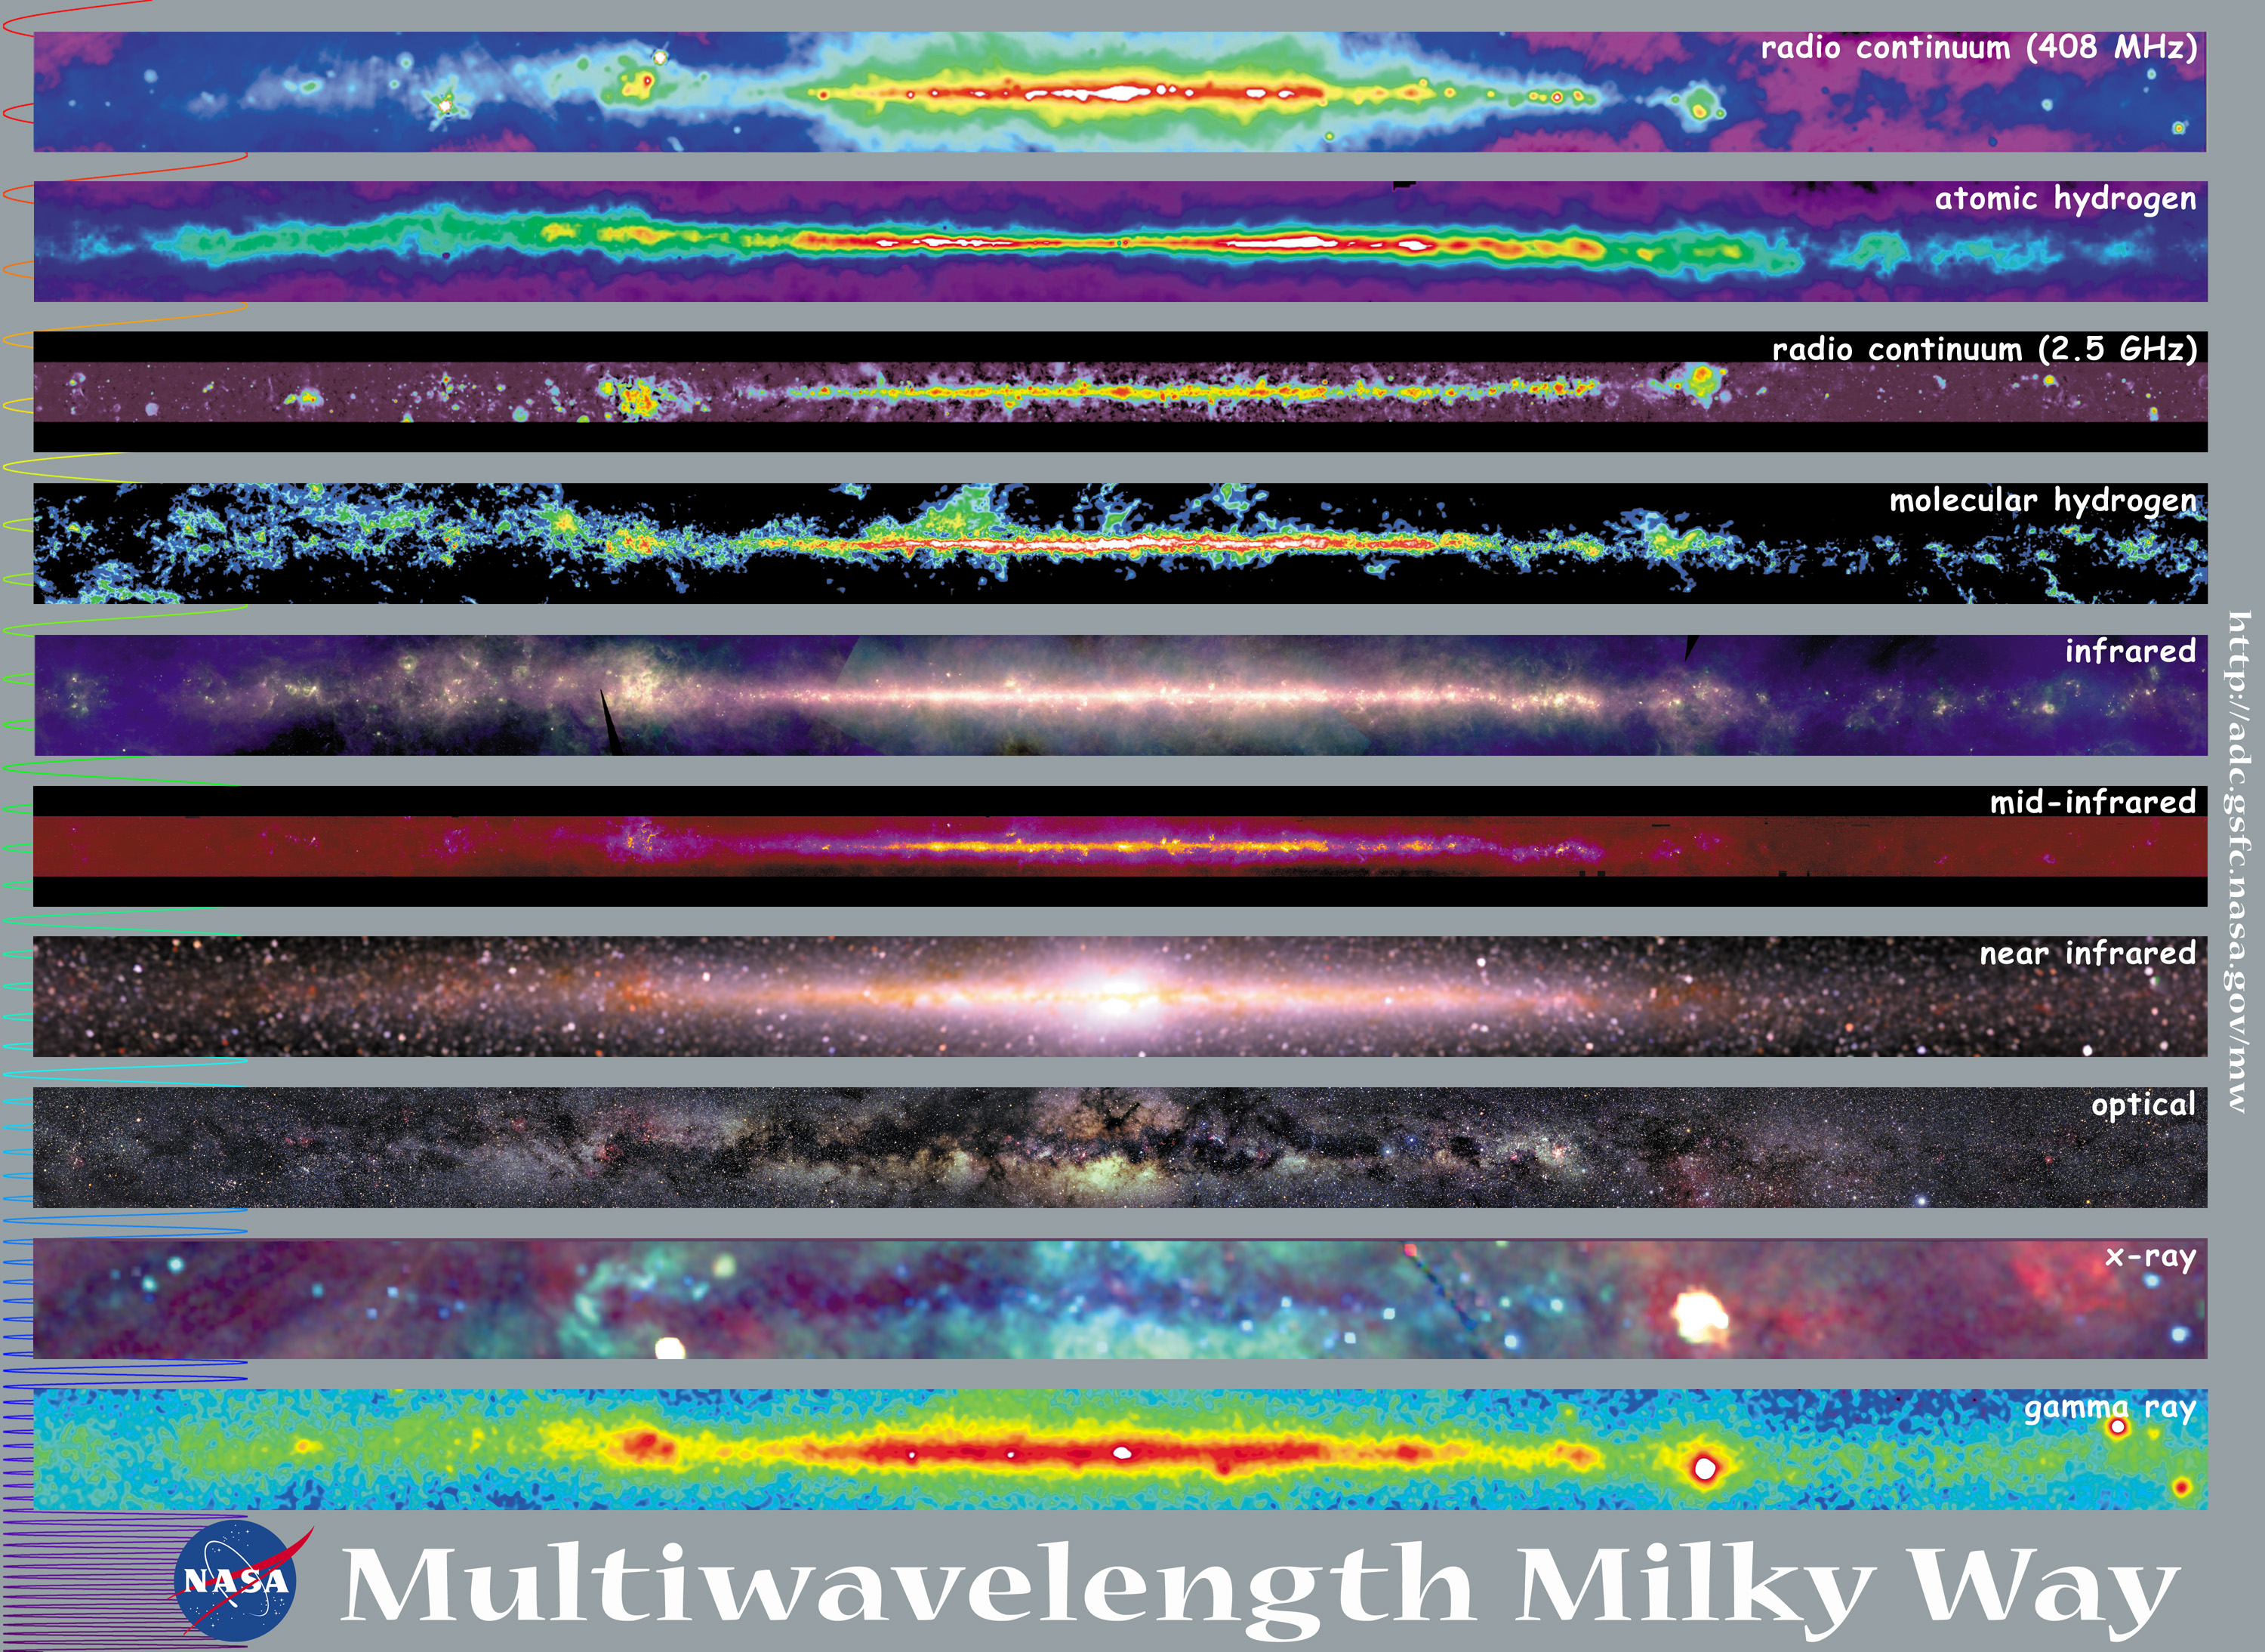
\includegraphics[width=\textwidth]{MW_morphology.jpg}
\end{center}
\end{figure}

Starting from the bottom and working back up:

Gamma rays:  The central plane of the galaxy is brightest at these wavelengths.  This radiation can come from objects such as blazers, pulsars, and accreting black holes, found predominantly in the mid plane of the galaxy.

X-rays:  Here the galaxy has a large scale height since the hot gas producing the x-rays has a larger scale height than the dust in the disk.  Dust is responsible for absorbing light from the mid plane.

Optical:  Most of the light comes from the mid plane and the central part of the bulge.  Since dust preferentially extincts bluer wavelengths, some light from the mid plane is extinct (this is coming from the young, bright, blue stars).

Near-IR:  As is evident from the image, there is hardly any extinction by dust in this wavelength range.  The light here is dominated by massive, evolved stars.  The bulge is especially bright since it s dominated by these evolved stars that peak in the near-IR.

Far-IR:  These wavelengths are dominated by reprocessed thermal emission from dust.  This emission is brightest at the mid plane.

Radio:  The continuum is dominated by synchrotron emission (from black holes, jets, pulsars, etc).  Objects producing this radiation are found in the mid plane - this it is bright in the radio.  In terms of line emission, hydrogen emission (21 cm line), is brightest at the mid plane but has a larger scale height than molecular gas that produces molecular lines.  

      
\item \textbf{Describe at least three methods to probe the gravitational potential of galaxies,
      their assumptions, and their realm of applicability.}
      
      Radial velocity curves of spiral galaxies: using the velocities measured by spectral lines at various radii in the galacy. Can be applied to spiral galaxies but not ellipticals or irregulars (I think)\sidenote{
        Michael -- I'm not sure this is true.  I think every galaxy has some rotational component
        and some velocity dispersion component.  Ellipticals have some coherent rotation as well.
        I just can't recall ever seeing a rotational velocity as a function of radius for a
        non-spiral galaxy.
      }. Here you're assuming Keplerian motion of the stars in the disk and that you can easily obtain disk velocities from the radial velocity by knowing how the galaxy's plane is projected on the sky.
      
      Velocity dispersions of ellipticals: here you can use the width of spectral lines to find the velocity distribution of stars. Limited to ellipticals (and maybe bulges of spirals?).
      
      Gravitational lensing: use the angle that light is gravitationally bent (corresponding to the Einstein radius) to measure the mass of a galaxy or galaxy cluster. Usually it's harder to get detailed information about the potential in space, since you'll normally just have one or a few lensed objects behind your foreground object. You also need to pick a foreground objects with lensable objects behind it.
      
\end{enumerate}

\subsection{``The Galaxy''}

Let's describe the strucutre of the Milky Way here.  I'll begin with the thick vs thin disk
because that's interesting to me.

\newthought{In 1983, Gilmore and Reid} noted two separate structures within the disk of the
Milky Way: the thin disk ($\sim1$ kpc scale height) and the thick disk
($\sim5$ kpc scale height).  The distinction (apart from the obvious difference in dynamics)
is that the thick disk consists of an older population of stars while the thin disk consists
of a younger population of stars.
The stars in the thick disk are believed to be have been formed in a thinner disk and then
excited to larger scale heights through encounters with satellite galaxies or mergers.
The thin disk is believed to have been formed by gas
accretion at later times during the formation of the galaxy.

I believe we had a colloquium earlier this year (or last year) that used SDSS data to show
that there is no thin disk/thick disk distinction but rather a continuous distribution
where the scale height of a stellar population scales with its age.

\subsection{The Luminosity Function}

The luminosity function $\Phi(M)dM$ is the number of objects per volume in an absolute magnitude range $M$ to $M+dM$. 

In the context of stars, note that while faint K and M dwarfs make up most of the stellar mass density in the solar neighborhood, almost all emitted light comes from the rare, luminous stars. The peak of the stellar luminosity function occurs at about $M_v = 12.5$, as a result of the rapid luminosity decline of main sequence stars as their mass approaches the limit of hydrogen burning ( $M_{crit} = 0.08 M_\odot$)

If the stars in a given population were born at different times, the stellar luminosity function must be corrected for the effects of stellar evolution. If the star formation rate is constant, as it is in the solar neighborhood,  the corrected luminosity function is given by:

 \begin{equation}
\Phi_0(M) = \Phi(M) \times
\begin{cases}
\frac{t}{\tau_{MS}(M)} & \text{for } \tau_{MS}(M)<t \\
1 & \text{otherwise}
\end{cases}
\end{equation} 
where $t$ is the time since formation started and $\tau_{MS}(M)$ is the main sequence lifetime of stars with absolute magnitude $M$. Note that we only observe stars of magnitude $M$ that were formed in the last $\frac{t}{\tau_{MS}(M)}$ fraction of the population's lifetime.

In the context of galaxies, the Schechter luminosity function provides a general analytic fit to galaxy functions. The Schechter function can be expressed in terms of luminosity:

\begin{equation}
\Phi(L) dL \propto L^\alpha  e^{\frac{-L}{L_*}} dL
\end{equation}
or in terms of absolute magnitude:

\begin{equation}
\Phi(M) dM \propto 10^{-0.4(\alpha+1)M} e^{-10^{0.4(M^*-M)}} dM.
 \end{equation}
 The parameters $\alpha$, $L^*$, and $M^*$ are usually fit to a given dataset. For galaxies near the Milky Way, $\alpha = -1$ and $M^*_B = -21$. For the Milky Way itself, $L_* = 3\times 10^{10} L_\odot$. In the Schechter function, $M^*$ and $L^*$ are also the characteristic values at which the number of galaxies falls off sharply. x 

\subsection{The Initial Mass Function}

After a burst of star formation, the number of stars in a mass range $\mathcal{M}$ to $\mathcal{M}+d\mathcal{M}$ is given by:

\begin{equation}
dN = N_0 \xi(\mathcal{M}) d\mathcal{M}
\end{equation}
where $\xi(\mathcal{M})$ is the number of stars of mass $\mathcal{M}$, and $N_0$ depends on the normalization of $\xi$. The IMF is normalized such that:

\begin{equation}
\int d\mathcal{M} \mathcal{M} \xi(\mathcal{M}) = \mathcal{M}_\odot
\end{equation}
Thus, $N_0$ is the number of solar masses created in a star formation burst. 

The IMF is assumed to be a power law with mass. This is justified because star formation proceeds through many orders of magnitude of densities and temperatures, so we expect the IMF is be a pretty featureless function. The power law must be chosen such that the IMF steepens with increasing mass. It is given by:

\begin{equation}
\xi  \propto \mathcal{M}^{-2.35}
\end{equation}
This power law, valid for $\mathcal{M} \geq 1\mathcal{M}_\odot$ is known as the Salpeter IMF.

The IMF can also be expressed in terms of the luminosity function:

\begin{equation}
\xi(\mathcal{M}) = \frac{dM}{d\mathcal{M}} \Phi_0 [M(\mathcal{M})]
\end{equation}
where M is absolute magnitude and $\mathcal{M}$ is mass. The function $M(\mathcal{M})$ can be found theoretically or observationally. It can be calculated using models of stellar atmospheres and main sequence stars of varying masses and metallicities. These models break down at $M(\mathcal{M}) \leq 0.6 M(\mathcal{M}_\odot)$ due to spectral deviation from black bodies. $M(\mathcal{M})$ can also be found using mass measurements of binary stars, although the data is generally sparse and noisy. 

\subsection{Malmquist Bias}

In any apparent magnitude-limited survey, intrinsically brighter objects will be overrepresented. The sample's true mean absolute magnitude is biased by the amount

\begin{equation}
\overline{\Delta M} = \left<M\right>_m - M_0
\end{equation}
where $\left<M\right>_m $ is the uncorrected mean absolute magnitude, and $M_0$ is the true mean absolute magnitude. 

The Malmquist bias $\overline{\Delta M}$ is calculated using $A(m)$, the total number of stars brighter than the apparent magnitude $m$, and $\sigma$, the dispersion in the absolute magnitude:
\begin{equation}
\overline{\Delta M} = \left<M\right>_m - M_0 = -\sigma^2 \frac{d ln A}{dm}.
\end{equation}
The function A(m) is defined as

\begin{equation}
A(m) = w\int^\infty_{-\infty} ds \Phi(M) s^2 \nu(s)
\end{equation}
where w is the solid angle and s is the distance. We probably won't have to use that expression on the qual, but it may be useful to note that $\Phi(M)$ is often approximated as a gaussian centered on $M_0$ with a standard deviation of $\sigma$. 

The Malmquist bias also allows for a more accurate calculation of the mean distance to a sample, given the distance modulus. For example, solving for distance in the equation $(m-M_m)-\overline{\Delta M} = 5log\left(\frac{D}{10} \right)$.

\subsection{G-dwarf problem}

The closed box model of chemical evolution predicts that one half of all stars near the sun have less than a third of the metallicity of the most metal rich stars.  Since the latter have metallicities comparable to that of the Sun, the closed box model implies that one half of solar neighborhood stars should have metallicities less than $\frac{1}{3}z_\odot$.  However, from observations only $2$\% of disk F and G stars in the solar neighborhood have $z < -.25 z_\odot$.  This contradiction between the standard close-box model and observation is known as the G-dwarf problem.  From observations, stars are more metal rich than predicted.

\subsection{Distance Measures}

Moving cluster method:

\begin{equation}
D = \frac{-\theta}{\dot \theta}v_r
\end{equation}

Measuring the radial velocity of the cluster and the rate at which the cluster is expanding or shrinking allows you to find the distance to the cluster.

Using proper motions:

\begin{equation}
v_t = v_rtan(\theta)
\end{equation}
\begin{equation}
v_t = \mu d
\end{equation}
\begin{equation}
\mu = \frac{v_rtan(\theta)}{d}
\end{equation}
\begin{equation}
d = \frac{v_rtan(\theta)}{\mu}
\end{equation}

Baade-Wessilink Method:

This method requires an expanding/shrinking object, for example a variable star or a type Ia supernova.  The change in the radius of the object is given by:

\begin{equation}
r_1 - r_2 = v_r(t_1 - t_2)
\end{equation}

Next, use the flux measured at each time to determine the ratio of the radii at those times.

\begin{equation}
F_1 = \frac{4\pi r_1^2\sigma T_1^4}{4\pi d^2}
\end{equation}

\begin{equation}
\frac{r_1}{r_2} = \bigg(\frac{F_1T_2^4}{F_2T_1^4}\bigg)^{\frac{1}{2}}
\end{equation}

Now you can solve for the radii individually, and use the angular size of the object to get the distance.  


\subsection{Star Formation}

Observational methods to measure star formation:

1.  UV continuum - the UV spectrum is dominated by young massive stars, SFR scales linearly with luminosity.
	
	pros:  directly linked to young stellar population, wide range in redshift explorable.
	
	cons:  sensitivity to extinction and the IMF
	
2.  Recombination lines:  young stars emit UV radiation that ionizes atoms (mostly H) in nearby gas clouds.  Free electrons in the ionized gas then recombine with atoms.  They then drop to less excited states.  

	pros:  direct and highly sensitive
	
	cons:  extinction, IMF, uncertainty in gas distribution
	
3.  far-IR continuum:  UV radiation from young stars can be absorbed by interstellar dust and reemitted in the thermal infrared.

	pros:  sensitivity
	
	cons:  not direct, atmospheric absorption, distribution of dust, contribution of old stars


\subsection{Galaxy Mass Measurements}

\begin{enumerate}
\item Mass to Light Ratio

Given measurements of a galaxy's flux and distance, the luminosity is calculated using $L=F 4\pi d^2$. A mass to light ratio is assumed to calculate the galaxy's mass. For spiral galaxies, $M/L$ is usually around 3-6$M_\odot/L_\odot$.

\item Kepler's Law

If a star can be observed orbiting a galaxy, its period $P$ and distance $a$ from the galactic center can be used to solve for the galaxy's mass using Kepler's law:
\begin{equation}
P^2 \propto \frac{a^3}{GM}.
\end{equation}
This is one of the most common methods of galaxy mass measurements\sidenote{
    Surely not.  This section is very misleading.  The period of a star orbiting a spiral
    galaxy is typically $\sim10$ Myr (guess, but it should be close).  What you actually care
    about is measuring the velocity dispersion (elliptical) or rotational velocity (edge-on
    spiral).  You need the distance to the galaxy, and \emph{then} you can get the mass.
    However, you do not measure the period.
}. 

\item Gravitational Lensing

The angle of deflection of a gravitationally lensed object is the angle between the stars actual position and the observed lensed position. It is given by:
\begin{equation}
\theta = \frac{4GM}{rc^2}.
\end{equation}
where the affected light rays are traveling at a distance r from the lens. The parameter r can be determined if the distance to the lens is known. Given a calculated value of r and an observed value of $\theta$, the mass M of the lens (in this case a galaxy) can be determined. This is the most accurate method of galaxy mass measurement.

\end{enumerate}

\subsection{Milky Way Formation Models}

Most of this section is based on UNM's astr422 website.

The first Milky Way formation models were based on the following observations of stellar populations:

\begin{enumerate}
\item Halo stars are old and metal poor
\item Disk stars are young and metal rich
\item High velocity stars near the sun are metal poor, have more eccentric orbits than most disk stars, have a high kinetic energy $E_z$ perpendicular to the disk, and have high angular momentum $L_z$. These characteristics are correlated with metallicity, in that lower metallicity implies high eccentricity and higher $E_z$. 
\end{enumerate}

\subsection{Eggen, Lynden-Bell, and Sandage 1962 (ELS)}

In a slowly varying potential, the orbital eccentricity, $E_z$, and $L_z$ are conserved (i.e. adiabatic). Therefore, metal-poor stars formed in eccentric orbits or the star formation history of the Milky Way was very violent. 

The ELS model claims that the Milky Way was formed from an spherical, rotating cloud of metal-poor gas. When the cloud exceeded the Jeans mass, it underwent free-fall collapse. Most of the metal-poor stars and globular clusters formed during this time, and were then ``left behind" in the halo as the cloud collapsed. Supernovae from this early stellar population increased the metallicity of the gas. The cloud continued to collapse into the metal-rich disk we see today, eventually forming the younger disk stars and clusters. This formation model is referred to as a ``top-down" process.

There are a number of problems with the ELS model:
\begin{itemize}
\item The MW would have needed a high initial star formation rate of 100-1000$M_\odot$/yr
\item No treatment of dark matter
\item The ELS does not explain the following (among other things)

\begin{itemize}
\item Thin/thick disk components
\item Age and metallicity differences in globular clusters
\item Retrograde motion of some halo stars
\item Some dynamical ``clumps," or moving groups, of halo stars
\end{itemize}

\end{itemize}

\subsection{Searle and Zinn 1978 (SZ)}

The SZ model suggests that the MW formed from the collapse and merging of individual gas clouds in a ``Bottom-up" process. These fragments were about the size of dwarf galaxies ($10^{6-8} M\odot$) or supergiant molecular clouds, and may have already formed some stars and globular clusters. The leftover fragments may have formed today's dwarf galaxies. 

By claiming that the galaxy formed out of many different components, the SZ model explains the retrograde motion and clumping behavior of some halo stars, as well as differing metallicities in halo globular clusters. 

As collisions between fragments heated the proto-galaxy, the collapse began to slow. This accounts for the age spread of halo and thick disk stars. Since $t_{ff} \propto \rho^{1/2}$, the collapse was the fastest where the density was highest. Since the density was highest in the innermost region of the proto-galaxy, the central bulge formed and underwent early chemical enrichment from SN. The bulge was further fed by dynamical friction, causing the massive fragments to slow down and spiral into the central bulge region. These predictions are confirmed by observations of old, metal-rich stars in the central bulge. 

The SZ model does not, however, include dark matter, or adequately explain the formation of the disk 

\subsection{Empirical Relations}

M-$\sigma$ relation:  Empirical correlation between the stellar velocity dispersion $\sigma$ of a galaxy bulge and the mass of the central supermassive black hole.

\begin{equation}
\frac{M}{10^8M\odot} = 1.9\bigg(\frac{\sigma}{200 \frac{km}{sec}}\bigg)^{5.1}
\end{equation}

Sersic's Law:  Describes how intensity of a galaxy varies with distance from the center.  

\begin{equation}
I(R) = I_0exp\bigg(-b_n\bigg(\frac{R}{R_e}\bigg)^{\frac{1}{n}} - 1\bigg)
\end{equation}

For elliptical galaxies n $\thicksim$ 4, and for spiral galaxies n is approximately 1.  $R_e$ is the radius of the isophote containing half the luminosity.  

Kormendy Relation:  Correlation between $R_e$ and $I_e$, the surface brightness at $R_e$.  

\begin{equation}
R_e \thicksim \bigg<I\bigg>_e^{-0.83}
\end{equation}

Faber-Jackson:  Relation between luminosity and the central velocity dispersion.

\begin{equation}
L \thicksim \sigma^4
\end{equation}

Tully Fisher Relation:  Empirical relation between the intrinsic luminosity of a spiral galaxy and its velocity width.

\begin{equation}
L \thicksim v_{rot}^4
\end{equation}

This relation enables the difficult to observe L to be calculated from $v_{rot}$.  The use of apparent brightness (observed) and the inverse square law allows the distance to objects to be estimated.  

\subsection{Toomre's Q parameter}

When are self-gravitating disks vulnerable to local gravitational instabilities?  Instabilities can arise from competition between gravity causing over dense regions to collapse, stellar dispersion which inhibits the collapse, and angular momentum which inhibits the collapse.  The condition for instability is Q $\textless$ 1, where Q is given by:

\begin{equation}
Q \thicksim \frac{\kappa \sigma}{3G\Sigma}
\end{equation}

In this equation, $\sigma$ is the stellar velocity dispersion, $\Sigma$ is the local surface density, and $\kappa$ is the epicyclic frequency (the frequency at which radially displaced particles will oscillate).

Marta will add the derivation when she is not hungry.





